\documentclass[10pt,a4paper]{article}
\usepackage[margin=1.8cm]{geometry}
\usepackage{newtxtext,newtxmath}
\usepackage{booktabs,tabularx,graphicx,subcaption,float,microtype}
\usepackage[colorlinks=true,allcolors=blue]{hyperref}
\hypersetup{
  pdftitle={Supplementary Material: Architecture and Preprocessing Choices under Dataset Shift in Single-Channel EEG Sleep Staging},
  pdfauthor={Ngo Nhat Quan; Pham Thai Son},
  pdfsubject={Supplementary material for an Informatics in Medicine Unlocked submission}
}
\renewcommand{\thetable}{S\arabic{table}}
\renewcommand{\thefigure}{S\arabic{figure}}
\newcommand{\mf}{\ensuremath{\mathrm{macro\text{-}F1}}}
\newcommand{\ci}{95\% CI}
\title{Supplementary Material\\\large Architecture and Preprocessing Choices under Dataset Shift in Single-Channel EEG Sleep Staging: A Controlled Evaluation on Sleep-EDF and SHHS1}
\author{Ngo Nhat Quan and Pham Thai Son}
\date{}

\begin{document}
\maketitle

This supplement contains implementation details and descriptive tables moved from the main manuscript.
The evidence labels are unchanged: seed 42 is primary, seed 123 is a post-protocol sensitivity repeat,
SHHS1 E1/E2 analyses are secondary on an opened cohort, and SHHS1 E3--E2/E4 analyses are post-hoc.
E6 estimates mean and standard deviation from each complete unlabelled target recording; it is label-free
but transductive at recording level, not purely inductive zero-shot inference.

\section*{Supplementary Methods S1: model and training details}

\subsection*{Architecture and feature construction}

Each encoder input is a 30-s epoch with 3,000 samples. The control encoder contains 15 separately
trained CNNs: three context groups (current, previous and next; C/P/N) crossed with five
class-specialised loss functions. Every CNN has a five-class output, not a binary head. Concatenating
its softmax outputs in C/P/N order gives 75 features per central epoch. The P and N inputs are shifted
within each recording and are trained against the central epoch's label; the first or last signal
epoch is replicated at a recording edge. No context crosses recording boundaries. These are
softmax-output features; their use does not imply that probability calibration has been established.

The ResNet-1D encoder instead produces a 128-dimensional, pre-dropout representation of the current
epoch. Layer specifications are given in Table~\ref{tab:sup_architecture}. Encoders are trained and
selected before sequence training. Their selected checkpoints are loaded in evaluation mode, and
features are cached without gradients. E1 reuses the E0 encoder and its features within the same
fold and seed; its sequence training settings differ from E0 (Table~\ref{tab:sup_training}). E1--E0
is therefore a sequence-model configuration comparison, not an architecture-only effect. E2--E1
replaces the feature/context package, including encoder training and selection, while retaining the
specified TCN recipe.

\begin{table}[H]
\centering\small
\caption{Layer specifications. Convolution entries give input/output channels, kernel, stride and
padding; $d$ denotes dilation. All final classifiers have five outputs.}
\label{tab:sup_architecture}
\begin{tabularx}{\textwidth}{p{2.5cm}X}
\toprule
Component & Layers and operations \\
\midrule
One control CNN & Conv1d $1\!\to\!10$, $k=55,s=1,p=27$, no bias; ReLU; batch
normalisation; max-pool $k=s=16$, ceiling mode. Then Conv1d $10\!\to\!5$,
$k=25,s=1,p=12$, no bias; ReLU; batch normalisation; the same max-pool.
Flatten $5\times12=60$; linear $60\!\to\!10$; ReLU; linear $10\!\to\!5$. \\
ResNet stem & Conv1d $1\!\to\!32$, $k=50,s=5,p=25$, no bias; batch normalisation;
ReLU; max-pool $k=3,s=2,p=1$. \\
ResNet blocks & Three residual blocks: $32\!\to\!64$ ($s=1$), $64\!\to\!128$
($s=2$), $128\!\to\!128$ ($s=2$). Each has two bias-free $k=7,p=3$ convolutions,
with the stated stride in the first and stride 1 in the second; batch normalisation after each,
ReLU after the first and after residual addition. Each shortcut uses a bias-free $k=1$ projection
with the first convolution's stride, followed by batch normalisation. \\
ResNet output & Global average pooling gives 128 features. During encoder training only,
dropout 0.5 precedes the linear $128\!\to\!5$ classifier. Cached features are taken before dropout. \\
BiLSTM & One bidirectional LSTM layer, input 75, hidden size 128 per direction;
linear $256\!\to\!5$ output. Packed sequences exclude batch padding from recurrence. \\
TCN & Linear input projection $75$ or $128\!\to\!128$; layer normalisation; GELU.
Six residual blocks, each with two bias-free $128\!\to\!128$ convolutions,
$k=3,s=1,p=d$, with $d\in\{1,2,4,8,16,32\}$. Each convolution is followed by
per-epoch layer normalisation, GELU and dropout 0.2. The shortcut is identity.
Final dropout 0.2 and linear $128\!\to\!5$. \\
\bottomrule
\end{tabularx}
\end{table}

\subsection*{Training and checkpoint selection}

All stages use the same subject partitions, with validation at the end of each epoch, but not the
same optimisation or selection rule. For a CNN specialised to class $c$, training counts $n_c$ and
$N=\sum_c n_c$ determine weighted five-class cross-entropy: the weight for $c$ is
$0.5/(n_c/N)$ and each other class has weight $0.5/((N-n_c)/N)$. These training-derived weights
are also used to evaluate its validation loss. ResNet uses weights $N/(5n_c)$, again computed only
from training subjects. Sequence-model cross-entropy is unweighted over valid labelled epochs.
CNN branch seeds are the campaign seed plus the branch index in C/P/N--stage order; ResNet and
sequence training use the campaign seed. No label smoothing, data augmentation or learning-rate
scheduler is used.

\begin{table}[H]
\centering\small
\caption{Specified training recipes. Patience counts end-of-epoch validation checks without an
improvement. E1 reuses the E0 encoder; all other reported encoder/sequence pairs are fitted for their
own input variant.}
\label{tab:sup_training}
\begin{tabularx}{\textwidth}{l*{4}{>{\raggedright\arraybackslash}X}}
\toprule
Setting & CNN15 (E0/E1) & BiLSTM (E0) & ResNet (E2--E6) & TCN (E1--E6) \\
\midrule
Optimiser & Adam & Adam & AdamW & Adam \\
Learning rate & $10^{-3}$ & $10^{-2}$ & $10^{-3}$ & $5\times10^{-4}$ \\
Weight decay & 0 & 0 & $10^{-4}$ & 0 \\
Batch size & 64 epochs & 4 recordings & 64 epochs & 8 recordings \\
Maximum epochs & 1,000 & 1,000 & 40 & 300 \\
Patience & 10 & 10 & 8 & 30 \\
Selected checkpoint & Minimum weighted validation loss & Maximum validation \mf &
Maximum validation \mf & Maximum validation \mf \\
Gradient-norm clipping & None & 1.0 & None & 1.0 \\
\bottomrule
\end{tabularx}
\end{table}

Whole retained recordings are the sequence units for training and inference. Batch padding and
unknown/movement labels are excluded from the loss and metrics; unknown epochs retain their
positions in the signal sequence. The TCN masks padded positions after the input projection and
each convolutional sub-block. Its theoretical receptive field is
$1+2(3-1)(1+2+4+8+16+32)=253$ feature epochs, spanning up to 126 epochs on each side, subject to
recording boundaries. This is not a causal architecture. E1 also receives the explicit neighbouring
signal epochs through its CNN features. The 100-epoch input used for timing below is a benchmark
shape, not a training-window length.

\subsection*{Signal operations and evaluation windows}

Signal values are read in physical microvolts. Sleep-EDF uses Fpz--Cz at 100 Hz. SHHS1 uses C4--A1
and is resampled continuously from 125 to 100 Hz with polyphase resampling (up/down = 4/5,
Kaiser window $\beta=5$, constant padding). Table~\ref{tab:sup_variants} specifies operations after
this cohort-specific loading/resampling step. Filtering uses a fourth-order Butterworth design
with 0.5--30 Hz cutoffs, implemented as second-order sections with forward--backward filtering.
It operates on the continuous recording before epoch extraction and trimming.

\begin{table}[H]
\centering\small
\caption{Input variants and fitted components. Operations are listed in execution order; all
model weights are learned on Sleep-EDF only.}
\label{tab:sup_variants}
\begin{tabularx}{\textwidth}{lXX}
\toprule
ID & Signal operations & Encoder and sequence configuration \\
\midrule
E0 & Raw microvolt signal & CNN15 C/P/N, then BiLSTM \\
E1 & Raw microvolt signal & Reused E0 CNN15 C/P/N, then TCN \\
E2 & Raw microvolt signal & Current-epoch ResNet, then TCN \\
E3 & Band-pass; clip at $\pm800\,\mu$V; divide by 100 & Current-epoch ResNet, then TCN \\
E4 & Band-pass & Current-epoch ResNet, then TCN \\
E5 & Band-pass; clip at $\pm800\,\mu$V & Input-identity audit; excluded from performance analysis \\
E6 & Band-pass; clip at $\pm800\,\mu$V; recording-wise $z$-score & Current-epoch ResNet, then TCN \\
\bottomrule
\end{tabularx}
\end{table}

For E6, mean and population standard deviation ($\mathrm{ddof}=0$) are calculated over the entire
filtered and clipped recording, including portions outside the later evaluation window. The
implementation rejects zero or non-finite standard deviation rather than adding an epsilon;
non-finite input/output signals are also rejected. Processing uses float64 for filtering and
normalisation and stores model inputs as float32. On SHHS1 this is label-free target-record
normalisation with a transductive dependency; it does not update model weights. E3 and E6 are
trained separately on their respective source input variants, so their comparison is not an
amplitude-only intervention on one frozen classifier.

The evaluation window extends up to 30 minutes before the first and after the last reference
sleep epoch (N1, N2, N3 or REM), clipped to recording limits. Original stage 3/4 labels are merged
as N3; unknown/movement epochs are unscored. This reference-dependent trimming convention and
the later boundary diagnostics must be distinguished from label-free model fitting/inference.
Sleep-EDF metrics use out-of-fold predictions, with each subject evaluated by a model not trained
on that subject. SHHS1 uses the arithmetic mean of class probabilities from all ten source-fold
models before argmax. Cross-cohort score differences therefore compare distinct cohorts and
evaluation settings, not an isolated effect of dataset shift.

\subsection*{Runtime measurement}

The archived forward-pass benchmark used the selected fold-00, seed-42 checkpoints on a Tesla
V100-PCIE-16GB GPU, Python 3.10.13, PyTorch 2.5.1+cu124, CUDA 12.4 and cuDNN 9.1. It used float32
synthetic input of shape $(1,100,1,3000)$, 20 warm-up passes and 100 timed repetitions in each of
three rounds, with model order varied across rounds and GPU synchronisation around timing.
Both encoder and sequence forward passes are included; disk I/O, preprocessing, feature-cache
serialization and training are excluded. Latency is the median of the recorded passes; memory
is the maximum peak allocated GPU memory, distinct from reserved or incremental memory. These
measurements characterise offline computation, not the time until future EEG needed by a
bidirectional model becomes available. Training-and-validation wall-clock times additionally
depend on the recipes and stopping rules in Table~\ref{tab:sup_training}.

\section*{Supplementary results}

\begin{table}[H]
\centering\small
\caption{Per-class Sleep-EDF metrics for E3 and E6 (seed 42). Differences are calculated before rounding.}
\label{tab:sup_edf_perclass}
\begin{tabular}{lrrrrrrr}
\toprule
Stage & E3 Prec. & E3 Rec. & E3 F1 & E6 Prec. & E6 Rec. & E6 F1 & $\Delta$F1 \\
\midrule
W & .9338 & .9271 & .9304 & .9391 & .9169 & .9279 & +.0026 \\
N1 & .5149 & .5410 & .5276 & .5032 & .5219 & .5124 & +.0152 \\
N2 & .8583 & .8447 & .8514 & .8401 & .8368 & .8385 & +.0130 \\
N3 & .8072 & .8097 & .8085 & .7160 & .7779 & .7457 & +.0628 \\
REM & .8274 & .8413 & .8343 & .8227 & .8197 & .8212 & +.0131 \\
\bottomrule
\end{tabular}
\end{table}

\begin{table}[H]
\centering\small
\caption{Pooled E3 confusion matrix on Sleep-EDF (rows: reference; columns: prediction).}
\label{tab:sup_edf_confusion}
\begin{tabular}{lrrrrr}
\toprule
 & W & N1 & N2 & N3 & REM \\
\midrule
W & 61{,}133 & 3{,}888 & 416 & 56 & 448 \\
N1 & 3{,}283 & 11{,}643 & 4{,}867 & 105 & 1{,}624 \\
N2 & 539 & 5{,}496 & 58{,}394 & 2{,}271 & 2{,}432 \\
N3 & 30 & 45 & 2{,}377 & 10{,}558 & 29 \\
REM & 483 & 1{,}542 & 1{,}984 & 90 & 21{,}736 \\
\bottomrule
\end{tabular}
\end{table}

\begin{table}[H]
\centering\small
\caption{Sleep-EDF pooled \mf\ under two fixed seeds. Seed 42 is primary; seed 123 is a
post-protocol sensitivity repeat. Differences are calculated before rounding.}
\label{tab:sup_edf_seeds}
\begin{tabular}{lrrr}
\toprule
Configuration & Seed 42 & Seed 123 & Difference \\
\midrule
E0 & .7754 & .7755 & +.0000 \\
E1 & .7802 & .7776 & -.0026 \\
E2 & .7835 & .7828 & -.0007 \\
E3 & .7904 & .7883 & -.0022 \\
E4 & .7891 & .7887 & -.0004 \\
E6 & .7691 & .7780 & +.0089 \\
\bottomrule
\end{tabular}
\end{table}

\begin{table}[H]
\centering\small
\caption{Seed sensitivity of the protocol-specified Sleep-EDF contrasts. Bootstrap intervals
describe differences in pooled \mf; Wilcoxon tests use paired subject-wise \mf. Holm correction
is applied to the four tests within each seed, not to the marginal bootstrap intervals.}
\label{tab:sup_edf_seed_contrasts}
\begin{tabular}{lll}
\toprule
Contrast & Seed 42: $\Delta$ [\ci], $p_{\rm Holm}$ & Seed 123: $\Delta$ [\ci], $p_{\rm Holm}$ \\
\midrule
E1--E0 & .004811 [$-.000915$, .010193], .1022 & .002188 [$-.002870$, .007043], .9130 \\
E2--E1 & .003251 [$-.002370$, .008808], .1036 & .005143 [$-.000571$, .011292], .2400 \\
E3--E2 & .006962 [.000305, .014520], .8989 & .005478 [$-.002611$, .015796], .9130 \\
E3--E6 & .021319 [.012179, .030698], .0012 & .010249 [.002435, .017989], .1313 \\
\bottomrule
\end{tabular}
\end{table}

\begin{table}[H]
\centering\small
\caption{Seed-123 wall-clock training and validation time (10 folds, sequential, same GPU).
E1 time covers sequence training only because its encoder and cached features are reused from E0.}
\label{tab:sup_seed123_runtime}
\begin{tabular}{lrr}
\toprule
Configuration & Total & Mean per fold \\
\midrule
E0: 15-CNN + BiLSTM & 33 h 35 min 36 s & 3 h 21 min 34 s \\
E1: 15-CNN + TCN & 14 min 17 s & 1 min 26 s \\
E2: ResNet-1D + TCN & 2 h 44 min 57 s & 16 min 30 s \\
E3: fixed scale & 3 h 16 min 40 s & 19 min 40 s \\
E4: band-pass & 2 h 55 min 56 s & 17 min 36 s \\
E6: record-wise $z$-score & 2 h 24 min 44 s & 14 min 28 s \\
\bottomrule
\end{tabular}
\end{table}

\begin{table}[H]
\centering\small
\caption{Seed-123 sensitivity and E4 extension on the same 180 SHHS1 participants.
These are post-protocol results on the previously evaluated cohort.}
\label{tab:sup_shhs_seed123}
\begin{tabular}{lrrrr}
\toprule
ID & Subject-mean \mf & Pooled \mf & Accuracy & $\kappa$ \\
\midrule
E0 & .5303 & .5785 & .6738 & .5420 \\
E2 & .5409 & .5858 & .6874 & .5597 \\
E3 & .5634 & .6031 & .7003 & .5772 \\
E4 & .5732 & .6147 & .7064 & .5869 \\
E6 & .5503 & .5865 & .6873 & .5552 \\
\bottomrule
\end{tabular}
\end{table}

\begin{table}[H]
\centering\small
\caption{Paired SHHS1 seed-123 extension. Differences and subject-cluster percentile
bootstrap intervals concern subject-mean \mf\ (10,000 resamples). Two-sided Wilcoxon $p$-values
are Holm-adjusted within this four-contrast extension, separately from the primary seed-42 family.
W/T/L denotes subjects with a positive/zero/negative paired difference.}
\label{tab:sup_shhs_seed123_paired}
\begin{tabular}{lrrrr}
\toprule
Contrast & $\Delta$ subject-mean \mf & \ci & $p_{\rm Holm}$ & W/T/L \\
\midrule
E4--E2 & +.0323 & [.0236, .0410] & $7.40\times10^{-13}$ & 135/1/44 \\
E3--E4 & -.0098 & [$-.0125$, $-.0073$] & $1.89\times10^{-10}$ & 56/1/123 \\
E3--E6 & +.0131 & [.0023, .0239] & .0085 & 111/0/69 \\
E3--E0 & +.0331 & [.0225, .0438] & $5.19\times10^{-9}$ & 131/0/49 \\
\bottomrule
\end{tabular}
\end{table}

\begin{table}[H]
\centering\small
\caption{Secondary and post-hoc SHHS1 paired contrasts (seed 42; 180 subjects).
Intervals are marginal 95\% paired subject-cluster percentile bootstrap intervals for the
subject-mean difference, with 10,000 resamples. The E1/E2 extension was specified before their
SHHS1 inference but after the cohort had been evaluated with E0/E3/E6. E3--E2 was specified
after their separate marginal results had been examined.}
\label{tab:sup_shhs_secondary_paired}
\begin{tabular}{lrrrr}
\toprule
Contrast & $\Delta$ subject-mean \mf & \ci & $p$ & W/T/L \\
\midrule
E1--E0 & +.00651 & [.00192, .01087] & $.00325^{a}$ & 108/0/72 \\
E2--E1 & -.01280 & [$-.02209$, $-.00350$] & $.01005^{a}$ & 80/0/100 \\
E3--E2 & +.04750 & [.03724, .05792] & $2.35\times10^{-17}$\,$^{b}$ & 147/0/33 \\
\bottomrule
\end{tabular}

\smallskip
\begin{minipage}{0.96\textwidth}\footnotesize
$^{a}$Two-sided subject-wise Wilcoxon, Holm-adjusted within the two-contrast E1/E2 extension
(bootstrap seed 2031). $^{b}$Unadjusted two-sided Wilcoxon for one separately specified post-hoc
comparison (bootstrap seed 2032); it is not part of either historical Holm family. The contrasts
compare specified pipeline configurations, not isolated architectural effects.
\end{minipage}
\end{table}

\begin{table}[H]
\centering\small
\caption{Per-class transfer of E3; Pred/True is the predicted-to-reference class count ratio,
not a measure of probability calibration. Differences are calculated before rounding.}
\label{tab:sup_perclass_transfer}
\begin{tabular}{lrrrrrrr}
\toprule
& \multicolumn{2}{c}{Sleep-EDF} & \multicolumn{4}{c}{SHHS1} & \\
Stage & F1 & Pred/True & Prec. & Rec. & F1 & Pred/True & $\Delta$F1 \\
\midrule
W & .9304 & .993 & .8823 & .8014 & .8399 & .908 & -.0905 \\
N1 & .5276 & 1.051 & .2528 & .5437 & .3451 & 2.151 & -.1824 \\
N2 & .8514 & .984 & .7394 & .7349 & .7372 & .994 & -.1143 \\
N3 & .8085 & 1.003 & .9440 & .2582 & .4055 & .273 & -.4030 \\
REM & .8343 & 1.017 & .6052 & .8939 & .7218 & 1.477 & -.1125 \\
\bottomrule
\end{tabular}
\end{table}

\begin{table}[H]
\centering\small
\caption{Pooled E3 confusion matrix on SHHS1 (rows: reference; columns: prediction).}
\label{tab:sup_shhs_confusion}
\begin{tabular}{lrrrrr}
\toprule
 & W & N1 & N2 & N3 & REM \\
\midrule
W & 29{,}638 & 4{,}481 & 1{,}171 & 21 & 1{,}672 \\
N1 & 874 & 3{,}807 & 601 & 3 & 1{,}717 \\
N2 & 2{,}348 & 5{,}947 & 56{,}063 & 324 & 11{,}605 \\
N3 & 78 & 39 & 16{,}674 & 5{,}888 & 127 \\
REM & 655 & 784 & 1{,}311 & 1 & 23{,}183 \\
\bottomrule
\end{tabular}
\end{table}

\begin{table}[H]
\centering\small
\caption{Per-class SHHS1 metrics for E3 and E2 (seed 42).
Differences are calculated before rounding.}
\label{tab:sup_shhs_e3_e2_perclass}
\begin{tabular}{lrrrrrrr}
\toprule
Stage & E3 Prec. & E3 Rec. & E3 F1 & E2 Prec. & E2 Rec. & E2 F1 & $\Delta$F1 \\
\midrule
W & .8823 & .8014 & .8399 & .8780 & .7275 & .7957 & +.0442 \\
N1 & .2528 & .5437 & .3451 & .2367 & .3528 & .2833 & +.0618 \\
N2 & .7394 & .7349 & .7372 & .7362 & .6937 & .7143 & +.0228 \\
N3 & .9440 & .2582 & .4055 & .9659 & .2496 & .3967 & +.0087 \\
REM & .6052 & .8939 & .7218 & .4886 & .9450 & .6442 & +.0776 \\
\bottomrule
\end{tabular}
\end{table}

\begin{table}[H]
\centering\small
\caption{Reference-label oracle on E3 predictions (seed 42). Each row corrects only the indicated
confusion-matrix cell. The percentage is relative to the observed pooled-score difference between
Sleep-EDF out-of-fold evaluation and SHHS1 ensemble evaluation, not an isolated domain-shift effect
or an estimate of achievable model performance.}
\label{tab:sup_oracle}
\begin{tabular}{lrr}
\toprule
Condition & \mf & Numerical gap recovered \\
\midrule
Observed E3 on SHHS1 & .6099 & --- \\
Correct N3$\rightarrow$N2 only & .7444 & .1345 (74.5\%) \\
Correct N2$\rightarrow$REM only & .6596 & .0497 (27.5\%) \\
E3 on Sleep-EDF & .7904 & --- \\
\bottomrule
\end{tabular}
\end{table}

\begin{table}[H]
\centering\small
\caption{Post-hoc reference-label boundary and stable-interior diagnostics.
Seed 123 reuses the same subjects and label-defined regions; it is a sensitivity repeat, not
an independent cohort. All metrics are pooled within each region.}
\label{tab:sup_boundary}
\begin{tabular}{lllrrrr}
\toprule
Cohort & Seed & ID & \shortstack{Boundary\\\mf} & \shortstack{Stable\\\mf} &
\shortstack{Boundary\\N3 recall} & \shortstack{Stable\\N3 recall} \\
\midrule
Sleep-EDF & 42 & E0 & .6179 & .8175 & .6121 & .9216 \\
Sleep-EDF & 42 & E3 & .6321 & .8346 & .6326 & .9316 \\
Sleep-EDF & 123 & E0 & .6181 & .8173 & .6174 & .9162 \\
Sleep-EDF & 123 & E3 & .6343 & .8299 & .6385 & .9285 \\
\addlinespace
SHHS1 & 42 & E0 & .4323 & .5959 & .0633 & .4008 \\
SHHS1 & 42 & E3 & .4689 & .6220 & .0733 & .3900 \\
SHHS1 & 123 & E0 & .4336 & .5957 & .0639 & .3885 \\
SHHS1 & 123 & E3 & .4605 & .6166 & .0656 & .3660 \\
\bottomrule
\end{tabular}
\end{table}

For a label change between consecutive valid epochs $j-1$ and $j$, where $j$ is the first epoch
with the new label, the boundary neighbourhood contains $\{j-1,j,j+1\}$ within the same contiguous
recording segment. Overlapping neighbourhoods are combined. Unknown-label gaps and recording
boundaries break contiguity. Stable-interior epochs are at least three epoch positions from
\emph{both} sides of every label change, using distance
$\min(|i-(j-1)|,|i-j|)$; segments without a change are stable. The two regions do not exhaust the
scored epochs: Sleep-EDF contains 43,237 boundary, 130,693 stable and 21,539 remaining epochs;
SHHS1 contains 44,744, 103,195 and 21,073, respectively. The remaining epochs are not simply the
distance-two bin, because the boundary neighbourhood is centred on the first new-label epoch.
These masks include all stage changes, not just N2--N3. Where persistent boundaries are reported
in the archived diagnostics, each side must contain at least three consecutive epochs of its
respective label. Region metrics retain the fixed five-class convention used in the main analysis.

E6 N3 recall is 0.2005 overall and 0.0721 in the same SHHS1 boundary neighbourhood (seed 42), compared with
0.2582 and 0.0733 for E3. These regions use reference labels on both sides and are offline diagnostics,
not direct measurements of physiological transitions or deployable detectors. Differences in class
composition between regions also preclude interpreting their score difference as an isolated effect
of proximity to a label change. N3 under-detection persists in SHHS1 stable interiors in both seeds.

\section*{Supplementary analyses: representation and context}

The representation analysis uses the same 1,000 held-out epochs per fold for E1 and E2: 200 per
stage, sampled without replacement with a round-robin allocation across available subjects
(sampling seed $42+\text{fold index}$). In each representation and fold separately, features are
standardised and projected onto 20 principal components; these transforms are fitted to the
sampled test features solely for this descriptive analysis, not fed back into the staging model.
Silhouette uses Euclidean distance in the resulting space and the reference stage labels. The
mean coefficient across ten folds is 0.2126 (SD 0.0356) for E1 and 0.1048 (SD 0.0229) for E2.
E1 consists of 75 softmax-output features, whereas E2 is an unconstrained 128-dimensional
representation; this difference and the analysis transforms prevent treating silhouette as a
like-for-like measure of downstream predictive utility.

For the context ablation, the pretrained E0 encoder and 75-dimensional input interface are
retained. Each removed feature dimension is replaced by its mean over valid labelled training
epochs in that fold; the same replacement vector is applied to training, validation and test.
TCN models are retrained for C, CP and CN with the specified E1 recipe and seed 42, while full
CPN reuses E1. Thus the intervention changes the information available during both fitting and
inference; it is not an inference-only deletion. The local protocol specifies the primary CPN--C
boundary contrast and two secondary contrasts, with Holm correction across those three
subject-wise Wilcoxon tests. Bootstrap intervals describe paired differences in pooled boundary
\mf\ under 10,000 subject-cluster resamples (seed 2028).

\begin{table}[H]
\centering\small
\caption{Context-group ablation within E1 (seed 42). C, P and N denote current, previous and next
epoch feature groups. Differences are calculated before rounding.}
\label{tab:sup_context}
\begin{tabular}{lrrrrr}
\toprule
Condition & Overall \mf & $\Delta$ vs C & Boundary \mf & $\Delta$ vs C & N1 F1 \\
\midrule
C & .777477 & --- & .619102 & --- & .5011 \\
CP & .777733 & +.000257 & .617686 & -.001416 & .5022 \\
CN & .781585 & +.004108 & .618895 & -.000207 & .5055 \\
CPN & .780230 & +.002753 & .620055 & +.000953 & .5115 \\
\bottomrule
\end{tabular}
\end{table}

For the protocol-specified CPN--C boundary comparison, $\Delta\mf=0.000953$, \ci\
$[-0.004588,0.006568]$ and Holm $p=1.000$ (36/78 subjects improved). Secondary CPN--CP and CPN--CN
intervals also include zero with Holm $p=1.000$. The result does not show that temporal context or P/N
information is useless; it only finds no detectable marginal benefit for this encoding in E1.

\begin{figure}[H]
\centering
\begin{subfigure}{0.48\textwidth}
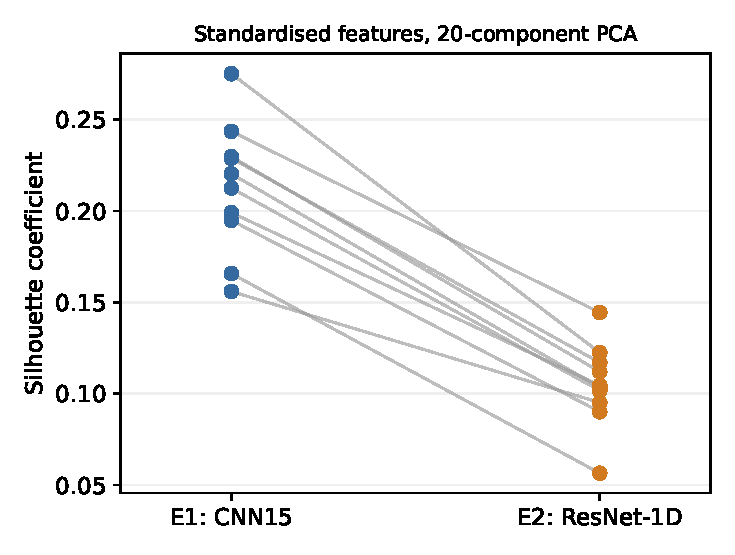
\includegraphics[width=\textwidth]{figures/gate8_feature_silhouette_en.pdf}
\caption{Silhouette by fold.}
\end{subfigure}\hfill
\begin{subfigure}{0.48\textwidth}
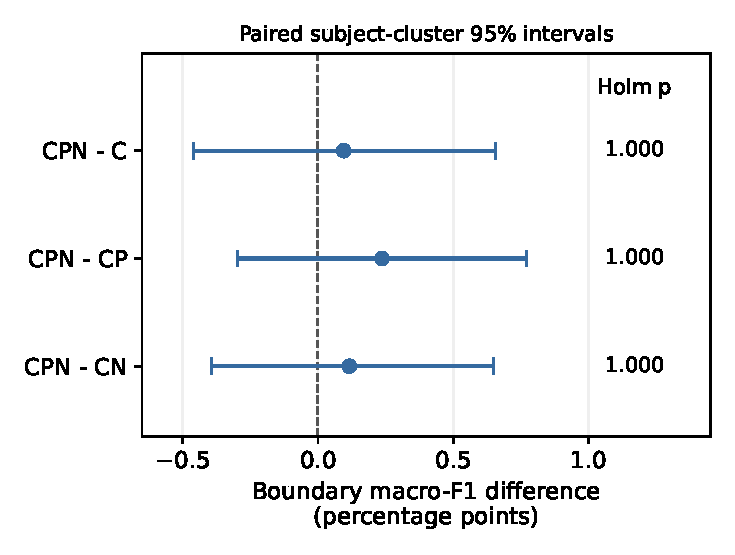
\includegraphics[width=\textwidth]{figures/gate8_context_ablation_effects_en.pdf}
\caption{Context-ablation effects.}
\end{subfigure}
\caption{Supporting representation and context analyses. (a) Silhouette coefficients by test fold. (b) Context-ablation effects showing paired 95\% confidence intervals of Boundary macro-F1 differences when ablating C/P/N context. All three paired intervals include zero and the Holm-adjusted Wilcoxon $p$-values are 1.000; no detectable marginal difference was observed for these contrasts within E1.}
\label{fig:sup_representation_context}
\end{figure}

\section*{Provenance}
\enlargethispage{4\baselineskip}

The historical SHHS protocol snapshot matches the original run-manifest hash
(`165d7cdf...fe93`); the expanded post-run audit (`9541e233...fe9`) does not replace it.
Table~\ref{tab:sup_boundary} reuses archived seed-123 diagnostics: source identities match the EDF
campaign and 20 E0/E3 fold-prediction files, and the SHHS1 extension manifest and 360 E0/E3 ensemble
files. Hash agreement establishes file identity, not an independent replication or public
preregistration. Raw SHHS data and predictions remain externally held; E6 is a descriptive
reanalysis of locked predictions. Snapshot paths and the reconciliation are documented in
\path{Reports/SHHS_PROTOCOL_PROVENANCE.md}.

\end{document}
